% atomic.tex
\documentclass{beamer}
\usetheme{Warsaw}
\author{Aditya Patawari, Lalatendu Mohanty}
\institute{
  Contributor to Fedora Project and Project Atomic\\[2ex]
  \texttt{aditya@adityapatawari.com}\\
  \texttt{lmohanty@redhat.com}\\
  \texttt{adimania on freenode irc}\\
  \texttt{http://blog.adityapatawari.com}
}
\title{Running your containers in a sane environment, Project Atomic}
\usepackage{graphicx}
\usepackage{ragged2e}
\usepackage{fancyvrb}
\usepackage[free-standing-units, space-before-unit, use-xspace]{siunitx}
\begin{document}

\begin{frame}
  \titlepage
  \end{frame}
\begin{frame}{Topics}
\begin{itemize}
  \item What is the problem?
  \item How Docker helps?
  \item Why not LXC containers or VM?
  \item Project Atomic is here!
  \item .. Along with some components
  \item Starting our Atomic Host
  \item Demo
\end{itemize}
\end{frame}

\begin{frame}{What is the problem?}
\begin{figure}[htp]
\centering

\includegraphics[scale=0.15]{problem.jpg}
\label{}
\end{figure}
\begin{itemize}
  \item My production needs to be homogeneous
  \item I need to ship entire environment to my colleague
  \item I need a stable environment to run containers
  \item I need to support automation
  \item Managing hosts should involve minimal efforts
\end{itemize}
\end{frame}

\begin{frame}{How Docker helps?}
\begin{figure}[htp]
\centering

\includegraphics[scale=0.30]{docker_logo.png}
\label{}
\end{figure}
\begin{itemize}
  \item Lightweight linux container
  \item Boots up in seconds
  \item Incrementally build, revert and reuse your container
  \item API to manage things remotely
\end{itemize}
\end{frame}

\begin{frame}{Why not LXC containers or VM?}
\begin{figure}[htp]
\centering

\includegraphics[scale=0.15]{fight.png}
\label{}
\end{figure}
\begin{itemize}
  \item Less resource consuming than virtual machines
  \item Faster than VM with reasonable amount of isolation. According to a benchmark by Boden Russell, IBM (approx figures):
  \begin{itemize}
    \item CPU usage 20\percent vs 70\percent
    \item Memory usage 50 MB vs 300 MB
  \end{itemize}    
  \item Better tools ecosystem around docker than LXC
  \item Case study of Spotify
\end{itemize}
\end{frame}

\begin{frame}{Project Atomic is here!}
\begin{figure}[htp]
\centering

\includegraphics[scale=0.25]{atomic_logo.png}
\label{}
\end{figure}
\begin{itemize}
  \item Minimal operating system
  \item Benefits of our favorite Enterprise Linux
  \item Robust atomic upgrades and systemd 
  \item Ready to take on cloud, virtualized or bare metal
\end{itemize}
\end{frame}

\begin{frame}{.. including rpm-ostree ..}
\begin{figure}[htp]
\centering

\includegraphics[scale=0.70]{Rpm_logo.png}
\label{}
\end{figure}
\begin{itemize}
  \item Bootable, immutable, versioned filesystem trees
  \item Composed from standard rpms
  \item Atomic upgrade and rollbacks
  \item Only /etc and /var are writable
\end{itemize}
\end{frame}

\begin{frame}{.. and Systemd ..}
\begin{figure}[htp]
\centering

\includegraphics[scale=0.45]{systemd.png}
\label{}
\end{figure}
\begin{itemize}
  \item System and service manager for Linux 
  \item Replacing the init in Centos 7
  \item Highly modular and much more powerful than sysV
  \item Check out http://0pointer.de/blog/projects/why.html
\end{itemize}
\end{frame}

\begin{frame}{.. also Introducing Cockpit..}
\begin{figure}[htp]
\centering
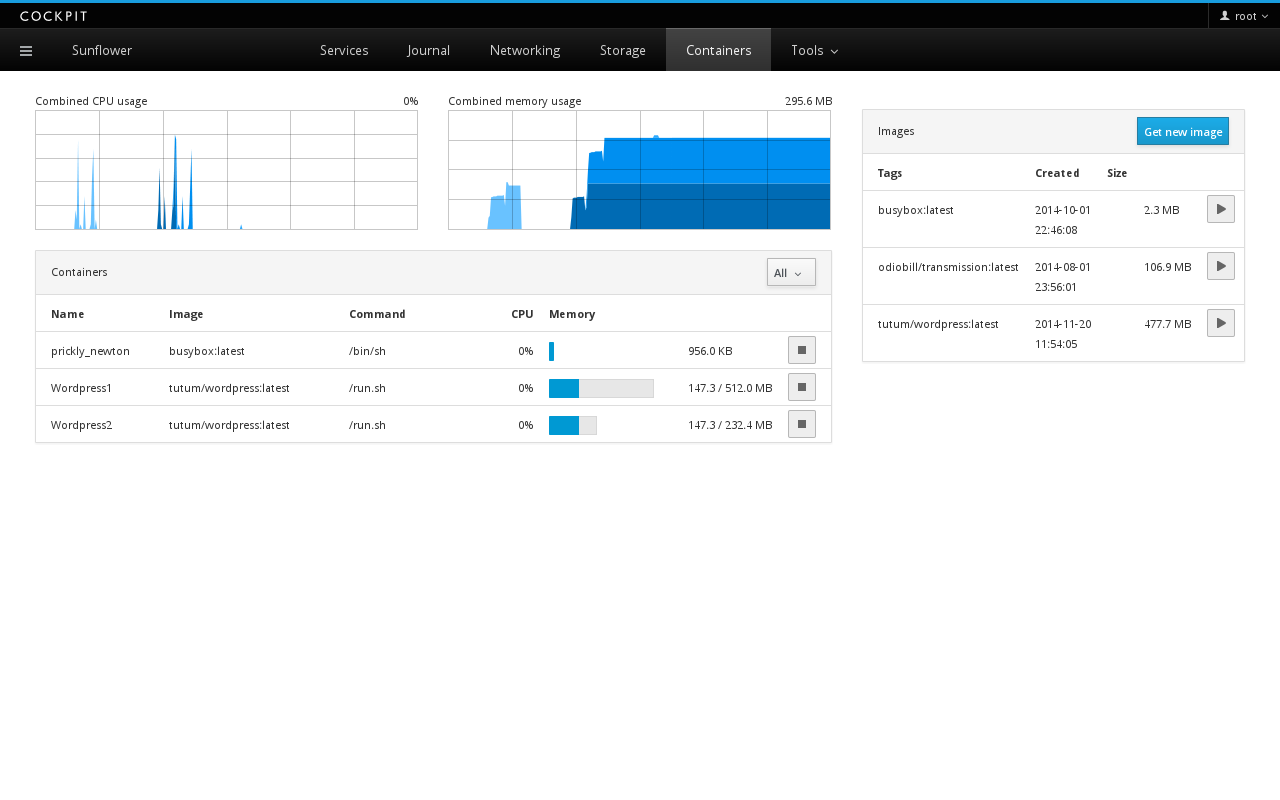
\includegraphics[scale=0.28]{cockpit.png}
\label{}
\end{figure}
\end{frame}

\begin{frame}{.. and lastly Kubernetes ..}
\begin{figure}[htp]
\centering

\includegraphics[scale=0.2]{kubernetes.png}
\label{}
\end{figure}
\begin{itemize}
  \item Master-slave arch
  \item Boot new containers
  \item Scalable and fault tolerant 
  \item Lots of examples and setup instructions at https://github.com/GoogleCloudPlatform/kubernetes
\end{itemize}
\end{frame}

\begin{frame}{Starting Atomic Host}
\begin{figure}[htp]
\centering
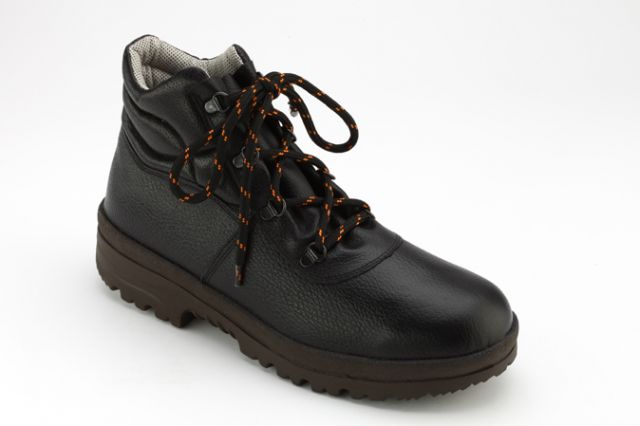
\includegraphics[scale=0.30]{boot.jpg}
\label{}
\end{figure}
\begin{itemize}
  \item Atomic host needs cloud-init data
  \item Info about the host, i.e. meta-data
  \item Info about the user, i.e. user-data
\end{itemize}
\end{frame}

\begin{frame}[fragile]
\frametitle{cloud-init data}
\begin{verbatim}
$ cat meta-data
instance-id: iid-local01;
local-hostname: myhost;

$ cat user-data
#cloud-config
password: mypassword
ssh_pwauth: True
chpasswd: { expire: False }

ssh_authorized_keys:
  - ssh-rsa ... foo@foo.com

$ genisoimage -output init.iso -volid cidata -joliet \
 -rock user-data meta-data
\end{verbatim}
\end{frame}

\begin{frame}{Demo!}
\begin{figure}[htp]
\centering

\includegraphics[scale=0.40]{demo.jpg}
\label{}
\end{figure}
\begin{itemize}
  \item Start a container.
  \item Verify that it works.
  \item Kill the container.
  \item OOOOO... Magic!
\end{itemize}
\end{frame}


\begin{frame}{Questions?}
Now is your chance :)
\end{frame}

\end{document}